\chapter{Experimental evaluation} % Main chapter title

\label{Chapter5} % For referencing the chapter elsewhere, use \ref{Chapter5} 

In this section, the experimental setup, the metrics for the evaluation between the three algorithms, as well as the result of the experiment are presented.

\section{Experimental Setup}
The main goal of this experiment is to measure how well the learning to rank algorithm is using the described dataset, taking the two remaining algorithms as the baseline. 

\noindent The two baseline algorithms used to compare with the learning to rank algorithm is the two that were mentioned in Chapter \ref{Chapter3}. The first one is the na\"ive collaborative filtering, which is the most simple and straightforward collaborative filtering method. The second one is the matrix factorization CF for implicit feedback dataset, which is the state-of-the-art collaborative filtering. The algorithm applies two different weighting strategies: one with a constant weighting scheme, while the other uses BM25 weight scheme \cite{singhal2001modern}.

\noindent For the ranking algorithm, two versions are setup: with and without item features. For the one with item features, the features are converted from continuous to categorical values, using the following rules:

\begin{itemize}
	\item Acousticness, danceability, energy, instrumentalness, liveness, speechiness, valence: the features are divided equally into 5 bins, each has range of 0.2.
	\item Key: each key represent a category on its own.
	\item Loudness: the feature is divided equally into 12 categories, each has range of 5.
	\item Tempo: tempo is categorized using standard Italian tempo markings \cite{2018Tempo}. In details, the feature is divided into these following categories:
	\begin{itemize}
		\item Grave: tempo from 40 to 50 beat per minute (bpm).
		\item Largo: tempo from 50 to 55 bpm.
		\item Larghetto: tempo from 55 to 60 bpm.
		\item Adagio: tempo from 60 to 70 bpm.
		\item Andante: tempo from 70 to 85 bpm.
		\item Moderato: tempo from 85 to 100 bpm.
		\item Allegretto: tempo from 100 to 115 bpm.
		\item Allegro: tempo from 115 to 140 bpm.
		\item Vivace: tempo from 140 to 150 bpm.
		\item Presto: tempo from 150 to 170 bpm.
		\item Prestissimo: tempo higher than 170 bpm.
\end{itemize}	  
\end{itemize}

As there are many hyperparameters in both implicit and ranking algorithm, a sequential optimization strategy using decision trees is used to optimize the hyperparameters \cite{ForestMinimize2018}. The model is improved by sequentially evaluating the expensive function at the next best point, thereby finding the best hyperparameters with as few evaluations as possible. 

To reduce the training time and approximate the best practice predicting time, instead of implementing the algorithms from scratch, I used a Python library developed by Benfred \cite{Benfred2018} for the implicit algorithm, and LightFM library \cite{DBLP:conf/recsys/Kula15} for the ranking algorithm.

\section{Score Metrics}
In this experiment, Average Precision (AP) is used to evaluate the efficiency of the algorithms. AP is defined as follow \cite{liu2009learning}:

\begin{displaymath}
AP(q) = \frac{\sum_{k=1}^m P@k(q) \cdot l_k}{\#\text{\{relevant documents\}}}
\end{displaymath}

\noindent with \( P@k \) is precision at K:

\begin{displaymath}
P@k(q) = \frac{\#\text{\{relevant documents in the top k positions\}}}{k}
\end{displaymath}

\noindent where \(m\) is the total number of document associated with query q, and \(l_k\) is the binary judgment on the relevance of the document at the \(k\)-th position. For this experiment, AP with value \(k = 1, 2, 3, 4, 5, \text{and } 10\) is measured, as we want to observe the behavior of the algorithms on optimizing for the top items. 

\section{Experiment Result}
The Average Precision of the algorithms is demonstrated in figure \ref{AP_result}. The na\"ive collaborative filtering has the poorest performance among the algorithms, with the Average Precision being 0.25 when \(k = 1\) and decreases to 0.2 when \(k = 5\), while the other two algorithms show comparable results. The learning to rank algorithm, optimizing for top items, has a slightly better precision compare to the implicit algorithm for \(k = 1 \text{and } 2\). As \(k\) increases, the precision of all algorithms declines. 

\noindent Adding music features from Spotify does not help increasing the accuracy of the algorithm. 

\begin{figure}[h]
	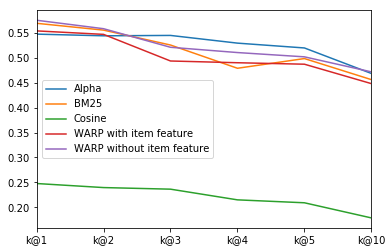
\includegraphics[width=8cm]{result}
	\centering
	\caption{Average Precision of the algorithms}
	\label{AP_result}
\end{figure}


